\documentclass[11pt,preprint]{elsarticle}

\usepackage{lmodern}
%%%% My spacing
\usepackage{setspace}
\setstretch{1.2}
\DeclareMathSizes{12}{14}{10}{10}

% Wrap around which gives all figures included the [H] command, or places it "here". This can be tedious to code in Rmarkdown.
\usepackage{float}
\let\origfigure\figure
\let\endorigfigure\endfigure
\renewenvironment{figure}[1][2] {
    \expandafter\origfigure\expandafter[H]
} {
    \endorigfigure
}

\let\origtable\table
\let\endorigtable\endtable
\renewenvironment{table}[1][2] {
    \expandafter\origtable\expandafter[H]
} {
    \endorigtable
}


\usepackage{ifxetex,ifluatex}
\usepackage{fixltx2e} % provides \textsubscript
\ifnum 0\ifxetex 1\fi\ifluatex 1\fi=0 % if pdftex
  \usepackage[T1]{fontenc}
  \usepackage[utf8]{inputenc}
\else % if luatex or xelatex
  \ifxetex
    \usepackage{mathspec}
    \usepackage{xltxtra,xunicode}
  \else
    \usepackage{fontspec}
  \fi
  \defaultfontfeatures{Mapping=tex-text,Scale=MatchLowercase}
  \newcommand{\euro}{€}
\fi

\usepackage{amssymb, amsmath, amsthm, amsfonts}

\def\bibsection{\section*{References}} %%% Make "References" appear before bibliography


\usepackage[numbers]{natbib}

\usepackage{longtable}
\usepackage[margin=2.3cm,bottom=2cm,top=2.5cm, includefoot]{geometry}
\usepackage{fancyhdr}
\usepackage[bottom, hang, flushmargin]{footmisc}
\usepackage{graphicx}
\numberwithin{equation}{section}
\numberwithin{figure}{section}
\numberwithin{table}{section}
\setlength{\parindent}{0cm}
\setlength{\parskip}{1.3ex plus 0.5ex minus 0.3ex}
\usepackage{textcomp}
\renewcommand{\headrulewidth}{0.2pt}
\renewcommand{\footrulewidth}{0.3pt}

\usepackage{array}
\newcolumntype{x}[1]{>{\centering\arraybackslash\hspace{0pt}}p{#1}}

%%%%  Remove the "preprint submitted to" part. Don't worry about this either, it just looks better without it:
\makeatletter
\def\ps@pprintTitle{%
  \let\@oddhead\@empty
  \let\@evenhead\@empty
  \let\@oddfoot\@empty
  \let\@evenfoot\@oddfoot
}
\makeatother

 \def\tightlist{} % This allows for subbullets!

\usepackage{hyperref}
\hypersetup{breaklinks=true,
            bookmarks=true,
            colorlinks=true,
            citecolor=blue,
            urlcolor=blue,
            linkcolor=blue,
            pdfborder={0 0 0}}


% The following packages allow huxtable to work:
\usepackage{siunitx}
\usepackage{multirow}
\usepackage{hhline}
\usepackage{calc}
\usepackage{tabularx}
\usepackage{booktabs}
\usepackage{caption}


\newenvironment{columns}[1][]{}{}

\newenvironment{column}[1]{\begin{minipage}{#1}\ignorespaces}{%
\end{minipage}
\ifhmode\unskip\fi
\aftergroup\useignorespacesandallpars}

\def\useignorespacesandallpars#1\ignorespaces\fi{%
#1\fi\ignorespacesandallpars}

\makeatletter
\def\ignorespacesandallpars{%
  \@ifnextchar\par
    {\expandafter\ignorespacesandallpars\@gobble}%
    {}%
}
\makeatother


% definitions for citeproc citations
\NewDocumentCommand\citeproctext{}{}
\NewDocumentCommand\citeproc{mm}{%
\href{\#cite.\detokenize{#1}}{#2}\nocite{#1}}

\makeatletter
% allow citations to break across lines
\let\@cite@ofmt\@firstofone
% avoid brackets around text for \cite:
\def\@biblabel#1{}
\def\@cite#1#2{{#1\if@tempswa , #2\fi}}
\makeatother
\newlength{\cslhangindent}
\setlength{\cslhangindent}{1.5em}
\newlength{\csllabelwidth}
\setlength{\csllabelwidth}{3em}
\newenvironment{CSLReferences}[2] % #1 hanging-indent, #2 entry-spacing
{\begin{list}{}{%
	\setlength{\itemindent}{0pt}
	\setlength{\leftmargin}{0pt}
	\setlength{\parsep}{0pt}
	% turn on hanging indent if param 1 is 1
	\ifodd #1
	\setlength{\leftmargin}{\cslhangindent}
	\setlength{\itemindent}{-1\cslhangindent}
	\fi
	% set entry spacing
	\setlength{\itemsep}{#2\baselineskip}}}
{\end{list}}

\usepackage{calc}
\newcommand{\CSLBlock}[1]{\hfill\break\parbox[t]{\linewidth}{\strut\ignorespaces#1\strut}}
\newcommand{\CSLLeftMargin}[1]{\parbox[t]{\csllabelwidth}{\strut#1\strut}}
\newcommand{\CSLRightInline}[1]{\parbox[t]{\linewidth - \csllabelwidth}{\strut#1\strut}}
\newcommand{\CSLIndent}[1]{\hspace{\cslhangindent}#1}


\urlstyle{same}  % don't use monospace font for urls
\setlength{\parindent}{0pt}
\setlength{\parskip}{6pt plus 2pt minus 1pt}
\setlength{\emergencystretch}{3em}  % prevent overfull lines
\setcounter{secnumdepth}{5}

%%% Use protect on footnotes to avoid problems with footnotes in titles
\let\rmarkdownfootnote\footnote%
\def\footnote{\protect\rmarkdownfootnote}
\IfFileExists{upquote.sty}{\usepackage{upquote}}{}

%%% Include extra packages specified by user
\usepackage{colortbl}
\providecommand{\pandocbounded}[1]{#1}
\usepackage{chngcntr}
\counterwithout{figure}{section}
\counterwithout{table}{section}\usepackage{booktabs}
\usepackage{longtable}
\usepackage{array}
\usepackage{multirow}
\usepackage{wrapfig}
\usepackage{float}
\usepackage{colortbl}
\usepackage{pdflscape}
\usepackage{tabu}
\usepackage{threeparttable}
\usepackage{threeparttablex}
\usepackage[normalem]{ulem}
\usepackage{makecell}
\usepackage{xcolor}

%%% Hard setting column skips for reports - this ensures greater consistency and control over the length settings in the document.
%% page layout
%% paragraphs
\setlength{\baselineskip}{12pt plus 0pt minus 0pt}
\setlength{\parskip}{12pt plus 0pt minus 0pt}
\setlength{\parindent}{0pt plus 0pt minus 0pt}
%% floats
\setlength{\floatsep}{12pt plus 0 pt minus 0pt}
\setlength{\textfloatsep}{20pt plus 0pt minus 0pt}
\setlength{\intextsep}{14pt plus 0pt minus 0pt}
\setlength{\dbltextfloatsep}{20pt plus 0pt minus 0pt}
\setlength{\dblfloatsep}{14pt plus 0pt minus 0pt}
%% maths
\setlength{\abovedisplayskip}{12pt plus 0pt minus 0pt}
\setlength{\belowdisplayskip}{12pt plus 0pt minus 0pt}
%% lists
\setlength{\topsep}{10pt plus 0pt minus 0pt}
\setlength{\partopsep}{3pt plus 0pt minus 0pt}
\setlength{\itemsep}{5pt plus 0pt minus 0pt}
\setlength{\labelsep}{8mm plus 0mm minus 0mm}
\setlength{\parsep}{\the\parskip}
\setlength{\listparindent}{\the\parindent}
%% verbatim
\setlength{\fboxsep}{5pt plus 0pt minus 0pt}



\begin{document}



\begin{frontmatter}  %

\title{Loans And Credit Analysis}

% Set to FALSE if wanting to remove title (for submission)




\author[Add1]{Diaz Sangeve}
\ead{24991422@sun.ac.za}





\address[Add1]{Stellenbosch University, Stellenbosch, South Africa}

\cortext[cor]{Corresponding author: Diaz Sangeve}

\begin{abstract}
\small{
Lending Club loans default at a rate that is set, above all, by the
grade the lender already assigns. Using one million anonymised loans,
this report defines default as a loan charged off against one fully paid
and asks what truly drives it. Credit grade separates a seven percent
default rate at A from a fifty seven percent rate at G, a fifty point
gap that dwarfs every other factor. Loan term and debt to income add
real risk, while home ownership and employment length, the two pillars
of the Institute's heuristics, move default only modestly and largely as
a by product of grade. States differ by about thirteen points, yet most
of that gap is composition rather than culture, and Texas sits squarely
at the national average. The grading system works, the interest rate it
sets follows credit rather than age, and a debt to income cap near
twenty to twenty five gives the Director a clean tolerance dial.
}
\end{abstract}

\vspace{1cm}





\vspace{0.5cm}

\end{frontmatter}

\setcounter{footnote}{0}


\renewcommand{\contentsname}{Table of Contents}
{\tableofcontents}

%________________________
% Header and Footers
%%%%%%%%%%%%%%%%%%%%%%%%%%%%%%%%%
\pagestyle{fancy}
\chead{}
\rhead{}
\lfoot{}
\rfoot{\footnotesize Page \thepage}
\lhead{}
%\rfoot{\footnotesize Page \thepage } % "e.g. Page 2"
\cfoot{}

%\setlength\headheight{30pt}
%%%%%%%%%%%%%%%%%%%%%%%%%%%%%%%%%
%________________________

\headsep 35pt % So that header does not go over title




\newpage

\section*{Reading default risk in a million
loans}\label{reading-default-risk-in-a-million-loans}
\addcontentsline{toc}{section}{Reading default risk in a million loans}

A loan book is a record of promises, some kept and some broken. This
report reads the Lending Club extract the Director provided, one million
anonymised loans, and asks the plain question behind his mandate, which
borrowers fail to repay and why. The answer matters because the
Institute carries a set of long-held beliefs about who defaults, and the
Director wants them tested against the data rather than taken on faith.

The argument that follows has a single spine. Default in this portfolio
is, above almost everything else, a story about creditworthiness as the
lender already measures it. The grade Lending Club assigns at
origination separates the safe from the risky more sharply than any
borrower trait the Institute leans on, and once grade is on the table
the heuristics about home ownership, employment and state culture shrink
to the margins. The report builds that case factor by factor and closes
on what it means for assessing a borrower.

\section*{The data, and what counts as
default}\label{the-data-and-what-counts-as-default}
\addcontentsline{toc}{section}{The data, and what counts as default}

A loan only has a verdict once it has run its course. Following the
Director's own tip, default is defined on resolved loans, those that
were either paid in full or charged off as a loss, and the charged-off
loans are the defaults. Loans still marked Current are up to date and
tell us nothing yet, so they are set aside, as are the loans in
collections. Of the million loans, 597,668 are current and a further
19,130 sit in the partial-default band of late or grace-period payments,
the cases the recovery team is still working. That leaves 383,202
resolved loans, of which 86,079 were charged off, an overall default
rate of 22.5 percent.

\section*{What separates a defaulter}\label{what-separates-a-defaulter}
\addcontentsline{toc}{section}{What separates a defaulter}

The cleanest way to rank the drivers is to ask how far default moves
between the safest and the riskiest band of each factor. Table
\ref{drivertab} does exactly that, and the order is stark. Credit grade
opens a gap of 50.5 percentage points from its best band to its worst,
with interest rate next and itself little more than a restatement of
grade. Loan term and debt-to-income each move default by about fifteen
points, recent credit inquiries by a little less, and the factors the
Institute prizes sit lower down. Home ownership moves default by only
8.3 points, and the 9.4 points credited to employment length are
misleading, since almost all of that gap comes from loans with no
employment recorded rather than from tenure itself.

\begin{longtable}[t]{lr}
\caption{\label{tab:drivertab}\label{drivertab}Key risk drivers, ranked by the gap in default rate between their safest and riskiest band}\\
\toprule
Driver & Spread (pp)\\
\midrule
Credit grade & 50.5\\
Interest rate & 34.7\\
Recent inquiries & 32.6\\
Loan term & 15.4\\
Debt-to-income & 15.0\\
\addlinespace
Employment length & 9.4\\
Revolving use & 8.9\\
Home ownership & 8.3\\
Public records & 3.8\\
\bottomrule
\end{longtable}

Grade earns its place at the top because it behaves exactly as a grading
system should. Figure \ref{gradefig} shows default climbing without a
single reversal from 6.9 percent at A to 57.3 percent at G, a near
eightfold widening across the scale. By compressing dozens of
credit-file signals into one ordered letter, Lending Club hands an
assessor most of the predictive power in a single field, which is the
strongest single finding in the data and the anchor for the rest of the
report.

\begin{figure}[H]

{\centering 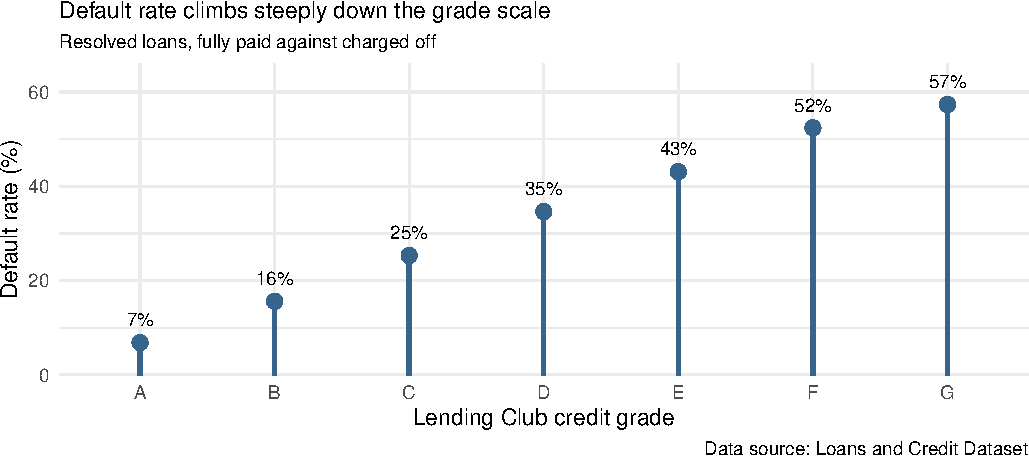
\includegraphics{Question3_files/figure-latex/gradefig-1} 

}

\caption{Default rate by Lending Club grade, resolved loans only.\label{gradefig}}\label{fig:gradefig}
\end{figure}

\section*{Which customers default
most}\label{which-customers-default-most}
\addcontentsline{toc}{section}{Which customers default most}

The question has layers, and the first layer is the one the Institute
states directly. Its belief is that home owners and borrowers employed
for more than ten years default far less often on short-term loans.
Restricting to the thirty-six month loans and crossing the two traits,
Table \ref{heurtab} shows the heuristic is half right and half
misdirected. Borrowers who both own property and have ten years of
tenure default 14.6 percent of the time against 20.3 percent for
everyone else, a real gap. The decomposition, though, shows the benefit
flows almost entirely from ownership. A renter with ten years of tenure
defaults at much the same rate as a renter without it, so employment
length on its own is close to noise.

\begin{longtable}[t]{llrr}
\caption{\label{tab:heurtab}\label{heurtab}Default on short-term (36 month) loans, by home ownership and employment length}\\
\toprule
Owns property & 10+ years employed & Default (\%) & Loans\\
\midrule
No & No & 23.2 & 92813\\
No & Yes & 23.0 & 28042\\
Yes & No & 17.2 & 107966\\
Yes & Yes & 14.6 & 68636\\
\bottomrule
\end{longtable}

Stacking the stronger drivers tells the fuller story of who fails to
repay. The deepest risk sits where a poor grade meets a sixty-month
term, the long loans the Director should watch, since term alone lifts
default from 19 percent on short loans to 34.5 percent on long ones.
Recent behaviour compounds it. Borrowers with no credit inquiry in the
last six months default near twenty percent, those with four or more
near thirty-five, and a borrower carrying a public record or running
their revolving credit to the limit adds several points again. The
riskiest customer is not defined by a demographic label but by a low
grade, a long term, a stretched debt load and a flurry of recent
credit-seeking.

\section*{The grading system and the price of
credit}\label{the-grading-system-and-the-price-of-credit}
\addcontentsline{toc}{section}{The grading system and the price of
credit}

The Director also asked whether grade predicts default for younger
borrowers and whether interest rates follow age, occupation and credit.
With no age field, the honest test uses credit-history length as a
proxy, and shorter histories do default more, rising from 20.3 percent
for borrowers with twenty or more years of history to 27 percent for
those with under five. Grade survives that test cleanly. Among borrowers
with less than ten years of history, the closest the data comes to the
young, default still rises from 7.2 percent at the A grade to 57.6
percent at G without a reversal, so the grade is a great indicator
regardless of how new the borrower is to credit.

The price of credit is settled almost entirely by that same grade. Table
\ref{irtab} lines the average interest rate up against the grade, and
the two move together at a correlation of 0.96, close to a straight
line. Interest rate is, in effect, a continuous restatement of the
grade. The claim that rates are determined by credit is therefore
strongly supported, since grade is the credit measure Lending Club uses,
while the parts of the heuristic that invoke age and occupation cannot
be tested and would in any case have little left to explain once grade
has done its work.

\begin{longtable}[t]{lr}
\caption{\label{tab:irtab}\label{irtab}Average interest rate by grade. The rate tracks the grade almost exactly}\\
\toprule
Grade & Mean interest rate (\%)\\
\midrule
A & 6.9\\
B & 10.2\\
C & 13.8\\
D & 18.2\\
E & 22.2\\
\addlinespace
F & 25.7\\
G & 28.8\\
\bottomrule
\end{longtable}

The claim that rates follow credit deserves to be seen rather than
asserted. Figure \ref{rateviolin} draws the distribution of interest
rate within each grade, and the violins step cleanly up the scale with
very little overlap between neighbours. A loan's grade fixes its price
to within a narrow band, which is the visual form of the near-perfect
correlation between the two and explains why the interest rate adds
almost nothing to grade as a separate signal.

\begin{figure}[H]

{\centering 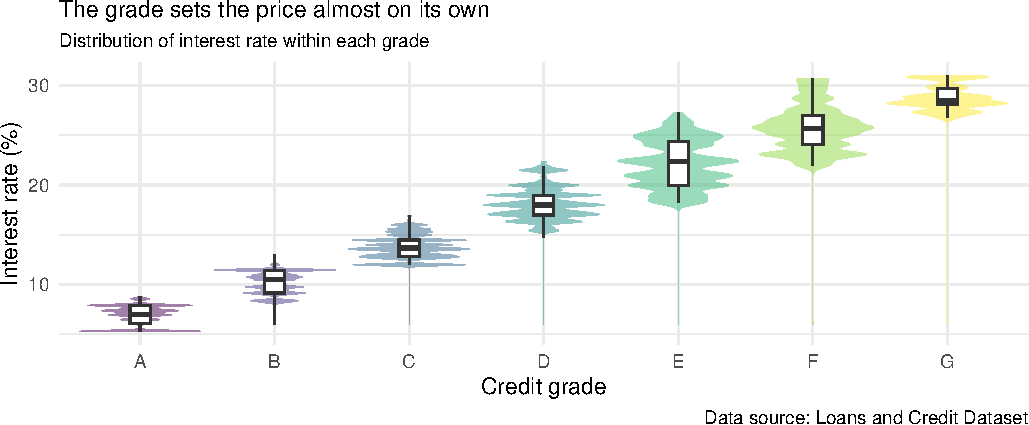
\includegraphics{Question3_files/figure-latex/rateviolin-1} 

}

\caption{Interest rate distribution within each credit grade.\label{rateviolin}}\label{fig:rateviolin}
\end{figure}

\section*{Where borrowers default, and whether Texas stands
apart}\label{where-borrowers-default-and-whether-texas-stands-apart}
\addcontentsline{toc}{section}{Where borrowers default, and whether
Texas stands apart}

States do differ, but less than the raw numbers suggest and less than a
story about culture would imply. Figure \ref{statefig} ranks the states,
and the spread runs from the low teens to the high twenties, a gap of
about thirteen points between the safest state and the riskiest. The
pattern has a geography to it, with the lowest rates in the Northeast
and Pacific Northwest and the highest across the Deep South, which is
the kind of regularity that tempts the word culture.

\begin{figure}[H]

{\centering 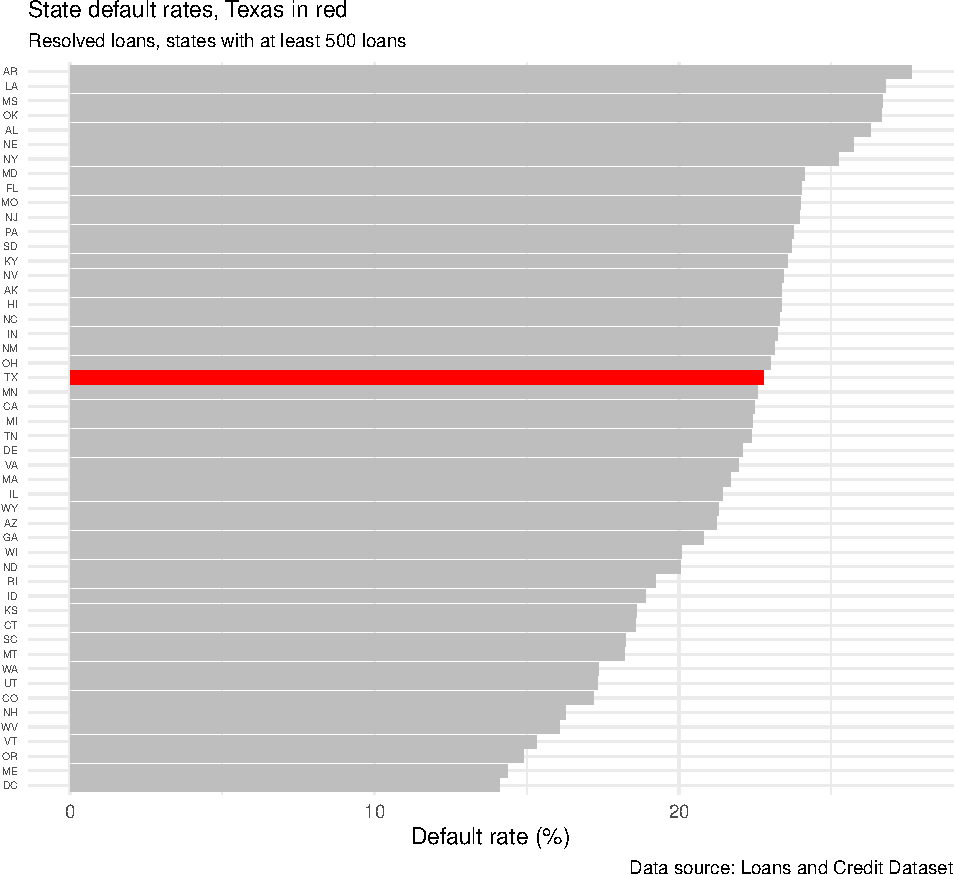
\includegraphics{Question3_files/figure-latex/statefig-1} 

}

\caption{Default rate by state, resolved loans, Texas highlighted in red.\label{statefig}}\label{fig:statefig}
\end{figure}

Most of that spread, though, is composition rather than culture. When
each state is measured against the default rate its own grade mix would
predict, the gaps narrow sharply. The Deep South still carries a genuine
excess of a few points above expectation, so a modest residual culture
effect may exist, but it is a fraction of the headline thirteen. Texas,
the Director's own state, is the clearest case of all. It defaults at
22.8 percent against a national rest near the same level, its
grade-adjusted excess is just 0.4 of a point, and it tracks the national
grade pattern almost exactly. On this evidence Texas is unremarkable,
neither a haven nor a hotspot, which is itself a useful thing for a
Texas director to know.

Putting the two strongest factors on one canvas settles how they
compare. Figure \ref{gradedtiheat} shows the default rate in every grade
and debt-to-income cell, with the number printed in each. Moving down
the grade axis shifts default far more than moving across the debt axis,
so within any debt band the grade still does most of the sorting, and a
high grade survives a high debt load better than a low grade survives a
low one.

\begin{figure}[H]

{\centering 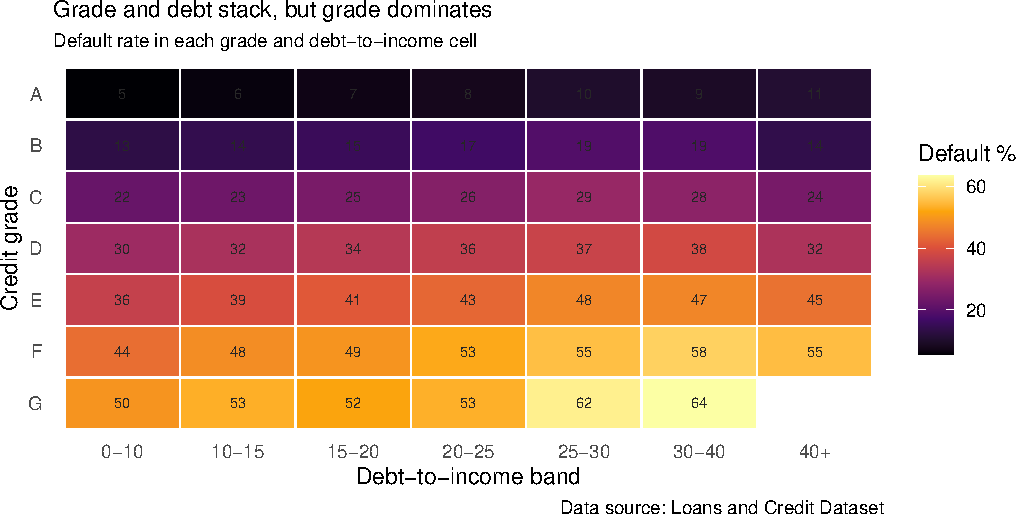
\includegraphics{Question3_files/figure-latex/gradedtiheat-1} 

}

\caption{Default rate by grade and debt-to-income band.\label{gradedtiheat}}\label{fig:gradedtiheat}
\end{figure}

\section*{A defensible debt-to-income
cap}\label{a-defensible-debt-to-income-cap}
\addcontentsline{toc}{section}{A defensible debt-to-income cap}

Debt-to-income is the lever the Director can actually pull at the point
of assessment, and the data gives it a clean shape. Figure \ref{dtifig}
shows default rising smoothly with the ratio, from under seventeen
percent in the lowest band to the low thirties at the top, with no cliff
edge that marks an obvious natural cap. Because the curve is smooth, the
right cap is a policy choice about tolerance rather than a number the
data dictates, so Table \ref{captab} turns it into a dial.

\begin{figure}[H]

{\centering 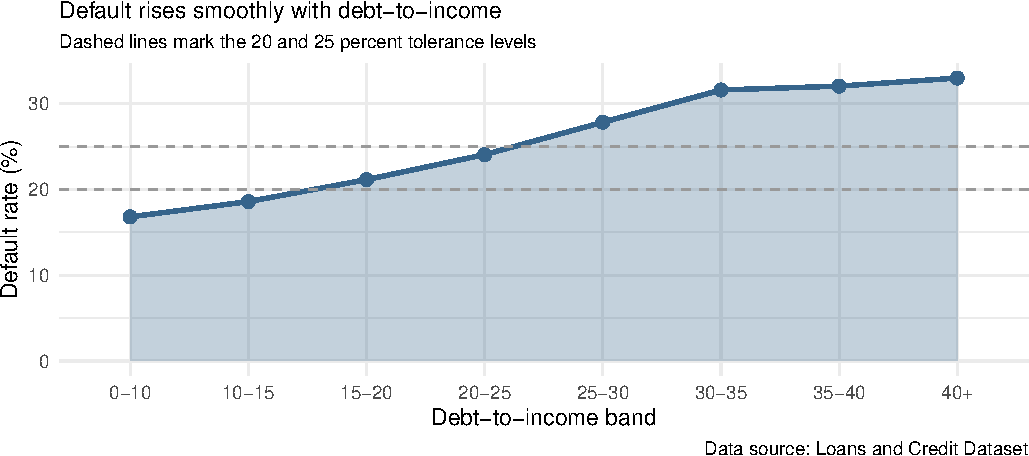
\includegraphics{Question3_files/figure-latex/dtifig-1} 

}

\caption{Default rate across debt-to-income bands, with the 20 and 25 percent tolerance lines.\label{dtifig}}\label{fig:dtifig}
\end{figure}

\begin{longtable}[t]{lr}
\caption{\label{tab:captab}\label{captab}Debt-to-income cap implied by each level of default tolerance}\\
\toprule
Default tolerance & DTI cap\\
\midrule
18\% & 10\\
20\% & 15\\
22\% & 20\\
25\% & 25\\
\bottomrule
\end{longtable}

A book willing to tolerate roughly a fifth of resolved loans defaulting
can lend up to a debt-to-income near twenty, while a more cautious book
aiming below that should draw the line closer to fifteen. Whether the
cap should move by state is a fair question, and the answer is a
qualified yes. The same high debt load carries very different risk
across states, with default above a debt-to-income of twenty running
near 16 percent in the safest state and above 32 in the riskiest, so a
lender could reasonably tighten the cap where the local book runs hot.
Texas again sits close to the national line, so a single national cap
would serve the Director's own state well enough.

The relationship between debt and default is worth fitting rather than
only banding. Figure \ref{dtilogit} shows a logistic regression of
default on the debt-to-income ratio, run separately for each term, so
the curve is the model's own estimate of risk rather than a histogram.
Default rises steadily with debt under both terms, and the sixty-month
curve sits clearly above the thirty-six-month one across the whole
range, which confirms that term and debt compound rather than cancel.

\begin{figure}[H]

{\centering 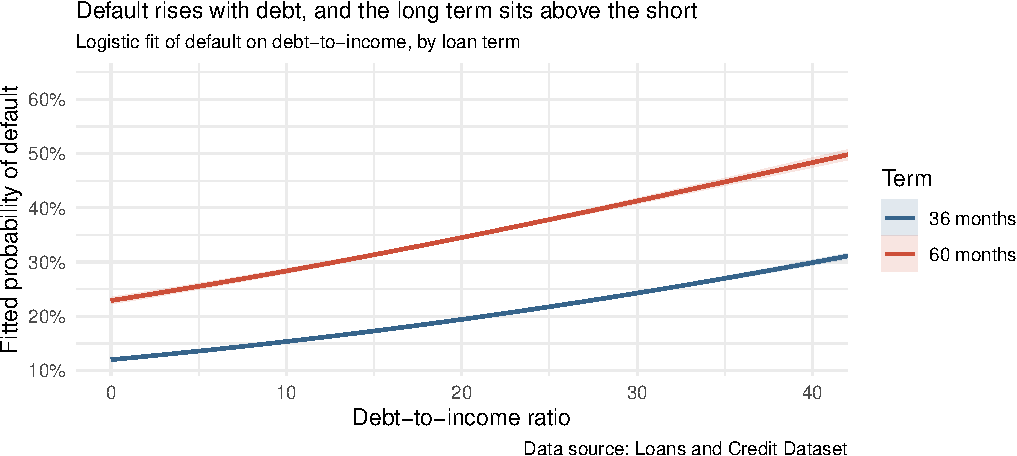
\includegraphics{Question3_files/figure-latex/dtilogit-1} 

}

\caption{Logistic fit of default probability on debt-to-income, by term.\label{dtilogit}}\label{fig:dtilogit}
\end{figure}

\section*{What this means for assessing a
borrower}\label{what-this-means-for-assessing-a-borrower}
\addcontentsline{toc}{section}{What this means for assessing a borrower}

Pulled together, the evidence points the Institute toward credit signals
and away from demographic ones. The grade already carries most of the
predictive weight, so the cheapest improvement an assessor can make is
to use it fully and to lean on the handful of behavioural fields that
add to it, namely the loan term, the debt-to-income ratio and the count
of recent credit inquiries. These are the levers that move default by
ten points or more, and three of them, term, debt and inquiries, can be
read straight off an application.

The Institute's three heuristics survive the data only in part. The
belief about home owners and long-tenured employees is half true, since
ownership does lower default modestly while employment length on its own
barely moves it, and both are small next to grade. The belief that
states differ by culture is mostly composition, real at the margin in
the Deep South but not the force the heuristic implies, and Texas is
ordinary. The belief that grade predicts default and that rates follow
credit is the one that holds firmly, with grade working even for the
newest borrowers and the interest rate set almost entirely by it. The
practical message is steady and slightly deflating for a book that
prizes its rules of thumb. The lender already holds the best predictor
it has in the grade, and the surest way to reduce default is to price
and cap against credit and debt rather than against the borrower's
address or years on the job.

\bibliography{Tex/ref}





\end{document}
